% AppD-Biology.tex

\clearpage

\chapter{BIOLOGICAL DATA}

These analyses have been performed on a GFBio extract dated 18 August 2014. We used the following data selection criteria for all the following analyses (the [agemeth] and [maturity] criteria were only used when the analyses required these data):

\section{Length and Weight Analyses}

After extracting all valid length/weight pairs of data based on the criteria shown in table~\ref{tab:bioCrit}, we used the following length-weight equation:

\begin{align} \label{eq:lw}
ln(W_i^s) = b^sln(L_i^s) + a^s + \varepsilon
\end{align}
\begin{addmargin}[3em]{1em}
where $a^s$ and $b^s$ are parameters for sex $s$ and $L_i^s$ and $W_i^s$ are paired length-weight observations.
\end{addmargin}

We only applied Equation~\eqref{eq:lw} to research or charter observations (trip\_type==2 or trip\_type==3) from PMFC areas 3CD5ABCDE. There were some bad data in the lower end of the distribution which possibly biased the analysis (Figure~\ref{fig:lwOptionA}). There are a number of ways to drop these data, including discarding large residuals (Option B: Table~\ref{tab:lwEst}, Figure~\ref{fig:lwOptionB}) or truncating the empirical distribution (We discarded the top and bottom 0.5\% of the distribution: Option C, Table~\ref{tab:lwEst}, Figure~\ref{fig:lwOptionC}). Finally, we combined the two truncation methods as Option D (Table~\ref{tab:lwEst}, Figure~\ref{fig:lwOptionD}). The models resulting from these three truncated analyses all appear to be effectively the same (see Figure~\ref{fig:lwCompare}) and the model using all the data is slightly to the right of the other three for both males and females. The parameter estimates for all four analyses were similar, although the exponent parameter is slightly lower for males and females for Option A (Table~\ref{tab:lwEst}). Option D had the best residual patterns (see Figure~\ref{fig:lwOptionD}) but all three truncated models will have the same impact when included in a biomass population model (Figure~\ref{fig:lwCompare}).  The model provided in Table 2 of \citet{arf2001} is similar to Option A for females but is to the left from the other four options for males (Figure~\ref{fig:lwCompare}).

\section{von-Bertalanffy Analyses}

We used the von-Bertalanffy function to estimate growth rates for \fishname:

\begin{align} \label{eq:vonb}
L_i^s = L_\infty^se^{(-k^s[a_i^s-t_0^s])}
\end{align}
\begin{addmargin}[3em]{1em}
where $L_\infty^s$, $k^s$, and $t_0^s$ are parameters specific to sex $s$ and $L_i^s$ and $a_i^s$ are paired length-age observations.
\end{addmargin}

There are several hundred paired length-age observations in most of the PMFC regions, except for 5A and 5E where the latter has no observations and the former has only a few (Table~\ref{tab:numagesByArea}). PMFC region 5D has about 3,000 age-length pairs which is the result of intensive sampling by the Hecate Strait multi-species assemblage survey. The maximum age of 50 in region 5B is the result of one male observation which was discarded because it was such a large outlier (model parameters were not affected by this single observation when fitted). The distributions by month are concentrated from late spring to mid-summer, with the large majority of the age-length pair originating from May and June (Table~\ref{tab:numagesByArea}). Using these data to estimate an annual growth rate is not ideal, but at least the observations are near mid-season. However, it is possible that this restricted seasonal distribution will lead to an underestimate of the growth rate.

The growth equations were calculated by combining the research and commercial data, and using all months from January to November (Table~\ref{tab:numagesByAreaMonth}). About two-thirds of the observations are from research and charter cruises but the addition of the extra 2,200+ observations from the commercial data has been done to obtain observations from months other than May and June. We calculated growth functions for 3CD as well as one for the combined 5ABCD (there were no 5E observations and relatively few 5A or 5B observations). The preferred model combines all data from the outside PMFC areas (3C to 5D and includes both the research and commercial data) (Figure~\ref{fig:vonb}) in order to obtain observations in months other than May and June. When the three investigated models are superimposed, the differences in estimated growth rates by sex are small, especially for females (Figure~\ref{fig:vonbCompare}). Males and females in 3CD have an  estimate that is \textgreater1 cm larger than for the other two models (Table~\ref{tab:vonbEst}). Males are about 10 cm smaller than females at the same age, which requires that this species should be modelled as with sexes separated (Figure~\ref{fig:vonbCompare}). The female growth function provided by \citet{arf2001} is very similar to the 3CD5ABD function calculated here but the male estimate is about 2-5 cm smaller than the estimates provided in Table~\ref{tab:vonbEst} (Figure~\ref{fig:vonbCompare}).

\section{maturity-at-age Analyses}

Before fitting models to the maturity data, we examined the available female \fishname staging information to ascertain the most likely period during which adult females would be in the reproductive phase (Table~\ref{tab:maturityMonth} and Figure~\ref{fig:maturity}). Given the information in Figure~\ref{fig:maturity}, it seemed most likely that the period over which females were mature extended from at least September to February, with Stage 3 females (Developing in Figure~\ref{fig:maturity}) at their most abundant from July to December and with Stage 4 and Stage 5 females appearing in January and February. The May and June data from the multi-species assemblage survey point to most of the fish being either immature or resting.  The progression of stages seemed consistent between observations generated from the research data and the commercial observers (compare left and right panels in Figure~\ref{fig:maturity}). This consistency between the two sets of observations is important because the amount of research data available to characterise this species is relatively sparse (see Table~\ref{tab:maturityMonth} and Table~\ref{tab:maturityObsPred}), requiring augmenting from the commercial data set.

We used stage 3 (Developing) and higher to define mature females, leaving stages 1 and 2 for immature \fishname. The number of mature females relative to the total number of valid otolith observations at each age was used as the data observation for each age (Equation~\ref{eq:matage1}). These proportions were fitted to a “double-normal” (half-Gaussian) function where the right-hand limb was constrained such that maturity equalled 1.0 when the age was greater than (Equation~\ref{eq:matage2}):

\begin{align} \label{eq:matage1}
P_a^f=N_a^{3-7}/N_a^{1-7}
\end{align}
\begin{addmargin}[3em]{1em}
where $P_a^f$ is the observed proportion mature at age $a_f$ calculated from the sum of valid observations at age for stages 3-7 ($N_a^{3-7}$) divided by the total number of staged females ($N_a^{1-7}$);
\end{addmargin}

\begin{align} \label{eq:matage2}
\hat{P}_a^f=
  \begin{cases}
    e^{\left(-\left(a^f-A^f\right)^2/e^{{\upsilon}L^f}\right)} & \text{if } a^f \leq A^f \\
                                              1 & \text{if } a^f > A^f
  \end{cases}
\end{align}
\begin{addmargin}[3em]{1em}
where $A^f$ and ${\upsilon}L^f$ are parameters for sex $f$ and $\hat{P}_a^f$ is the estimated proportion mature at age $a^f$;
\end{addmargin}

There were only 129 female age observations (of which only 3 were immature) with corresponding maturity data spanning the period July to February (see Table~\ref{tab:maturityObsPred}), leading to an estimated maturity curve that is not credible due to the lack of information at younger ages (Figure~\ref{fig:maturityfit}). More credible maturity ogives are generated with the addition of the May and June data, with little sensitivity to the inclusion or exclusion of the commercial observer data (Figure~\ref{fig:maturityOgiveCompare}). However, this ogive should be used with caution because it may be too spread out because of the difficulty of distinguishing between mature and immature fish at younger ages based on the macroscopic inspection of gonads.

It is not possible to compare this ogive with the one provided by \citet{arf2001} because their Figure 3 is a length-based maturity ogive. This figure would be based on the maturity information from the Hecate Strait Assemblage Survey, but this ogive would be sensitive to the same uncertainty in the maturity determinations as discussed in the previous paragraph.

% FIGURES
\begin{figure}[htp]
\captionsetup[subfigure]{labelformat=empty}
\begin{center}
\subfloat[]{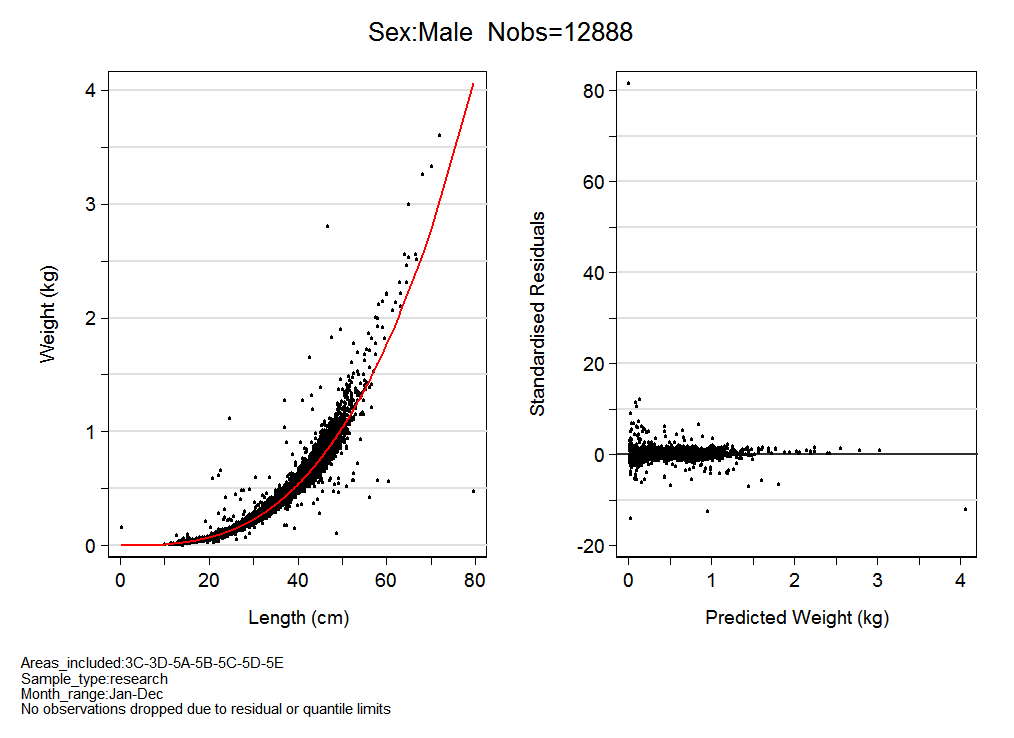
\includegraphics[bb=0 0 925 600,width=6in,keepaspectratio=true]{appD-Biology/lwmaleOptionA.png}}
\newline
\subfloat[]{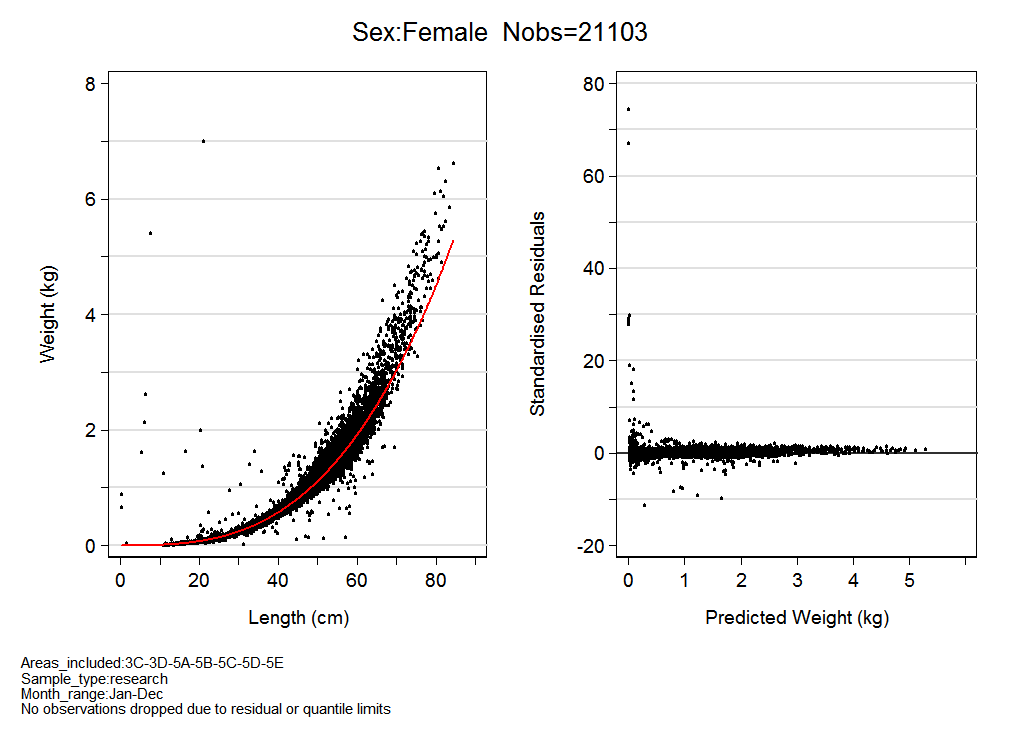
\includegraphics[bb=0 0 925 600,width=6in,keepaspectratio=true]{appD-Biology/lwfemaleOptionA.png}}
\end{center}
\caption{Length-weight plot for male [top panel] and female [bottom panel] \fishname: combined 3CD5ABCDE with no residual or distributional constraints (option A).}
\label{fig:lwOptionA}
\end{figure}

\begin{figure}[htp]
\captionsetup[subfigure]{labelformat=empty}
\begin{center}
\subfloat[]{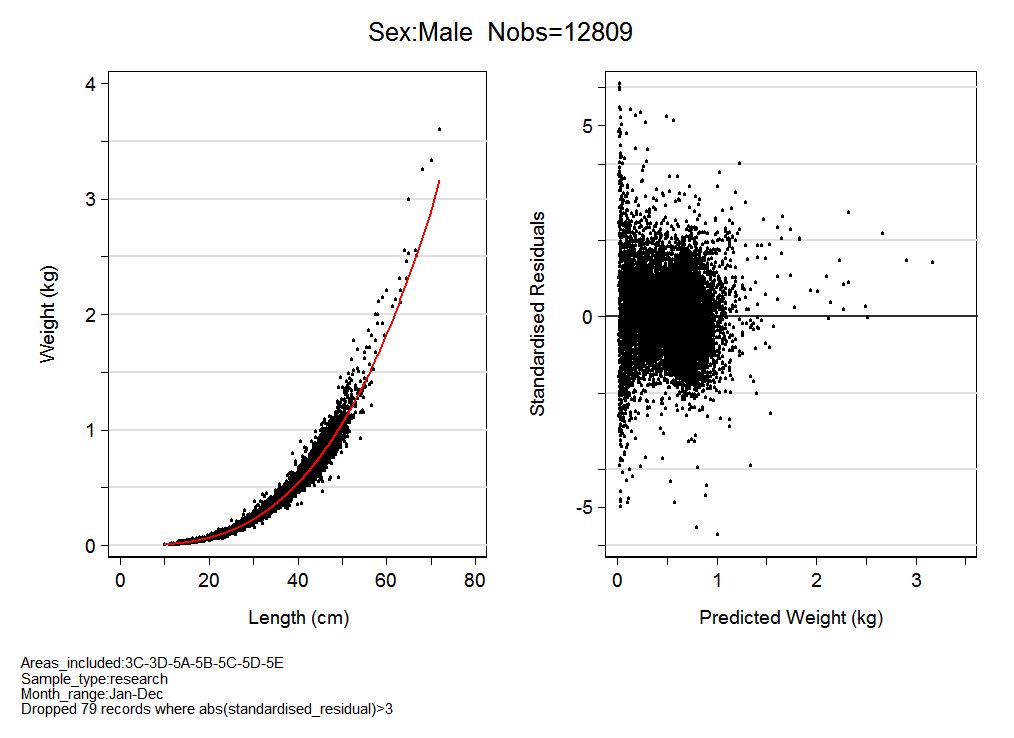
\includegraphics[bb=0 0 925 600,width=6in,keepaspectratio=true]{appD-Biology/lwmaleOptionB.png}}
\newline
\subfloat[]{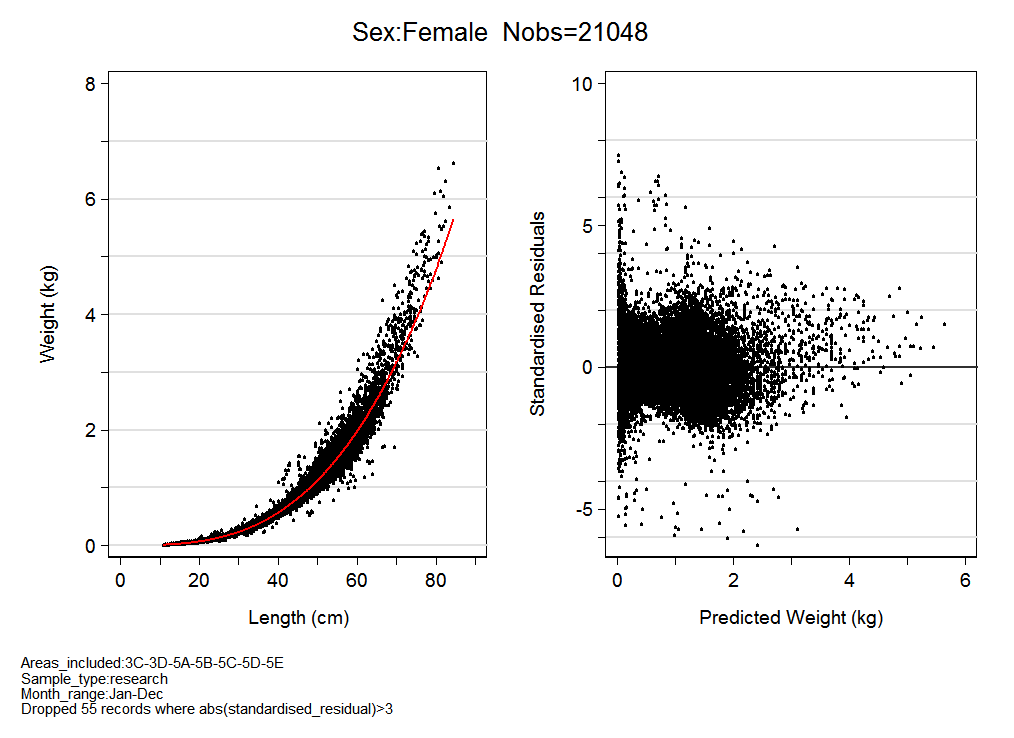
\includegraphics[bb=0 0 925 600,width=6in,keepaspectratio=true]{appD-Biology/lwfemaleOptionB.png}}
\end{center}
\caption{Length-weight plot for male [top panel] and female [bottom panel] \fishname: combined 3CD5ABCDE with no residual or distributional constraints but discarded standardised residuals (option B).}
\label{fig:lwOptionB}
\end{figure}

\begin{figure}[htp]
\captionsetup[subfigure]{labelformat=empty}
\begin{center}
\subfloat[]{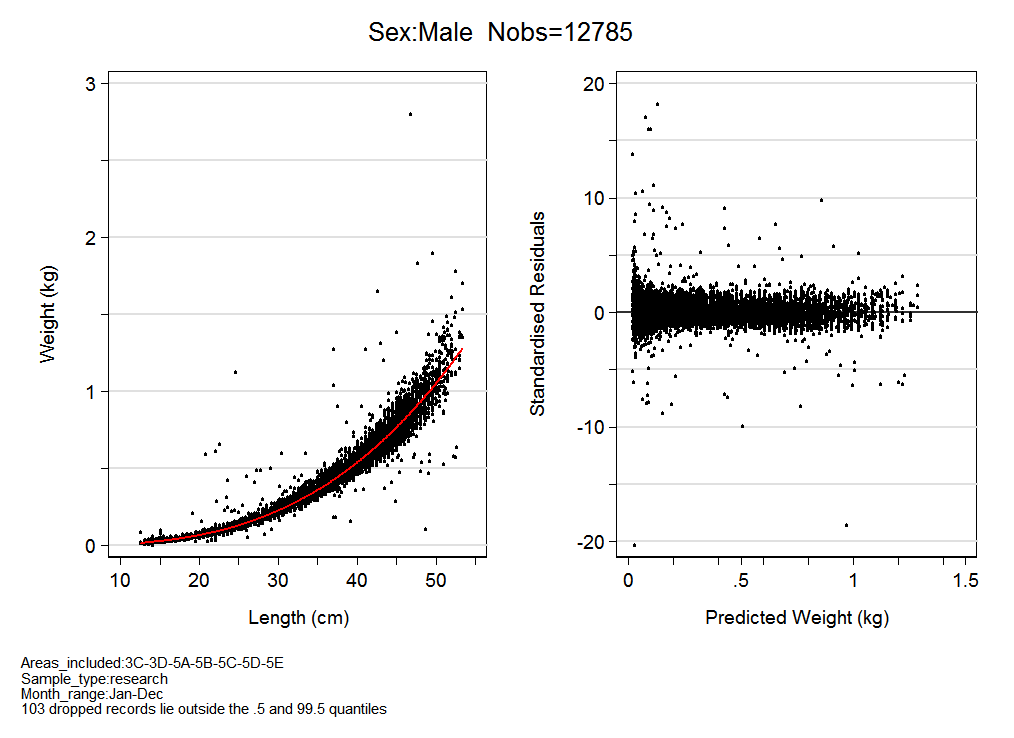
\includegraphics[bb=0 0 925 600,width=6in,keepaspectratio=true]{appD-Biology/lwmaleOptionC.png}}
\newline
\subfloat[]{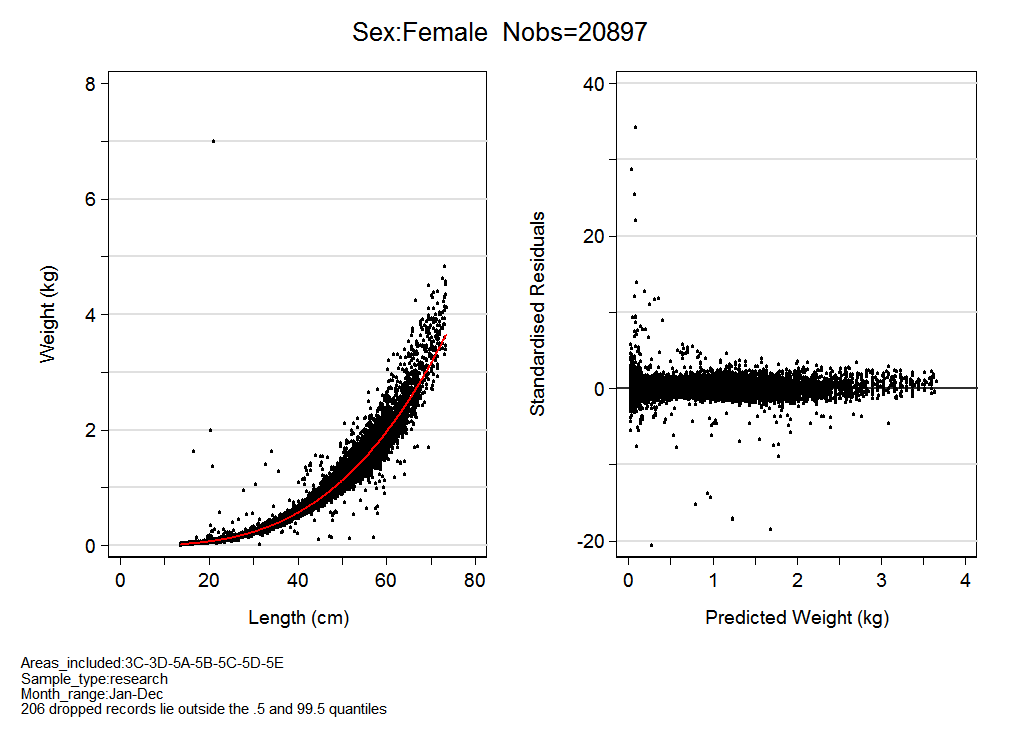
\includegraphics[bb=0 0 925 600,width=6in,keepaspectratio=true]{appD-Biology/lwfemaleOptionC.png}}
\end{center}
\caption{Length-weight plot for male [top panel] and female [bottom panel] \fishname: combined 3CD5ABCDE with no standardised residuals discarded but with the lower 0.5 and upper 0.95 quantiles of length dropped (option C).}
\label{fig:lwOptionC}
\end{figure}

\begin{figure}[htp]
\captionsetup[subfigure]{labelformat=empty}
\begin{center}
\subfloat[]{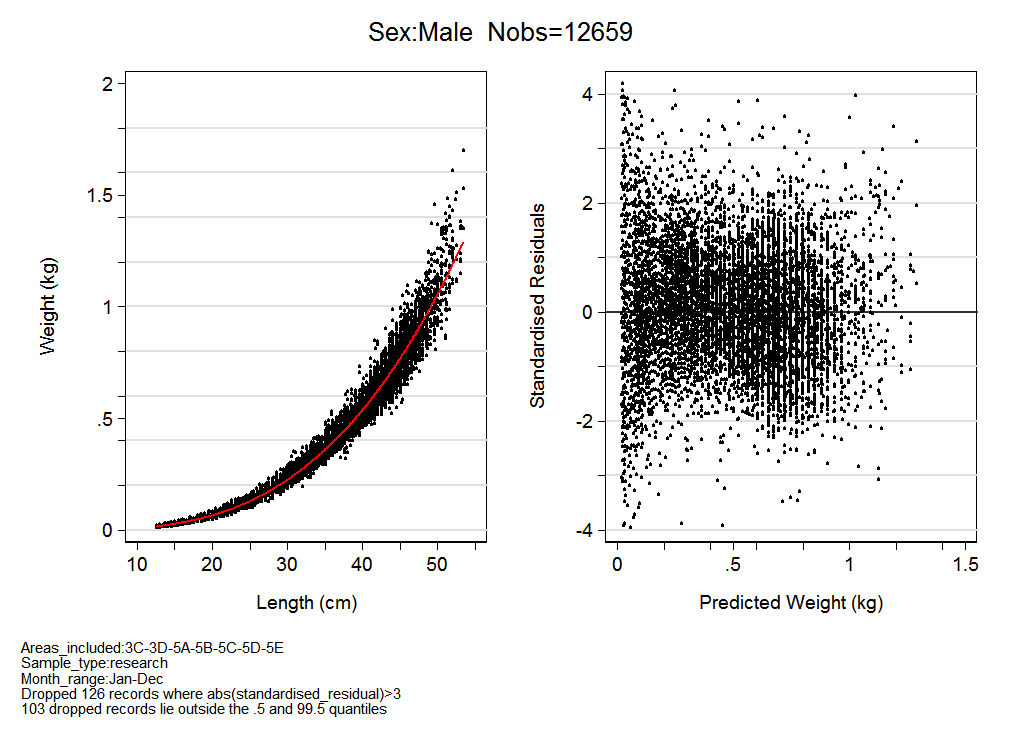
\includegraphics[bb=0 0 925 600,width=6in,keepaspectratio=true]{appD-Biology/lwmaleOptionD.png}}
\newline
\subfloat[]{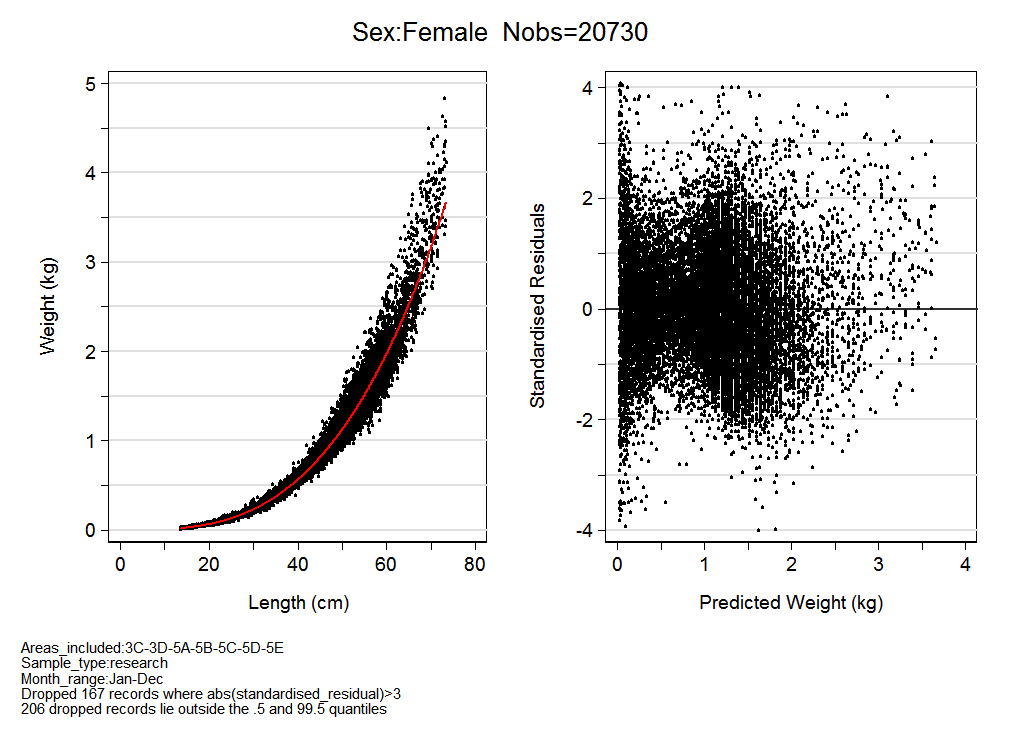
\includegraphics[bb=0 0 925 600,width=6in,keepaspectratio=true]{appD-Biology/lwfemaleOptionD.png}}
\end{center}
\caption{Length-weight plot for male [top panel] and female [bottom panel] \fishname: combined 3CD5ABCDE with standardised residuals \textgreater 3 discarded and with the lower 0.5 and upper 99.5 quantiles of length dropped (option D).}
\label{fig:lwOptionD}
\end{figure}

\begin{figure}[htp]
\captionsetup[subfigure]{labelformat=empty}
\begin{center}
\subfloat[]{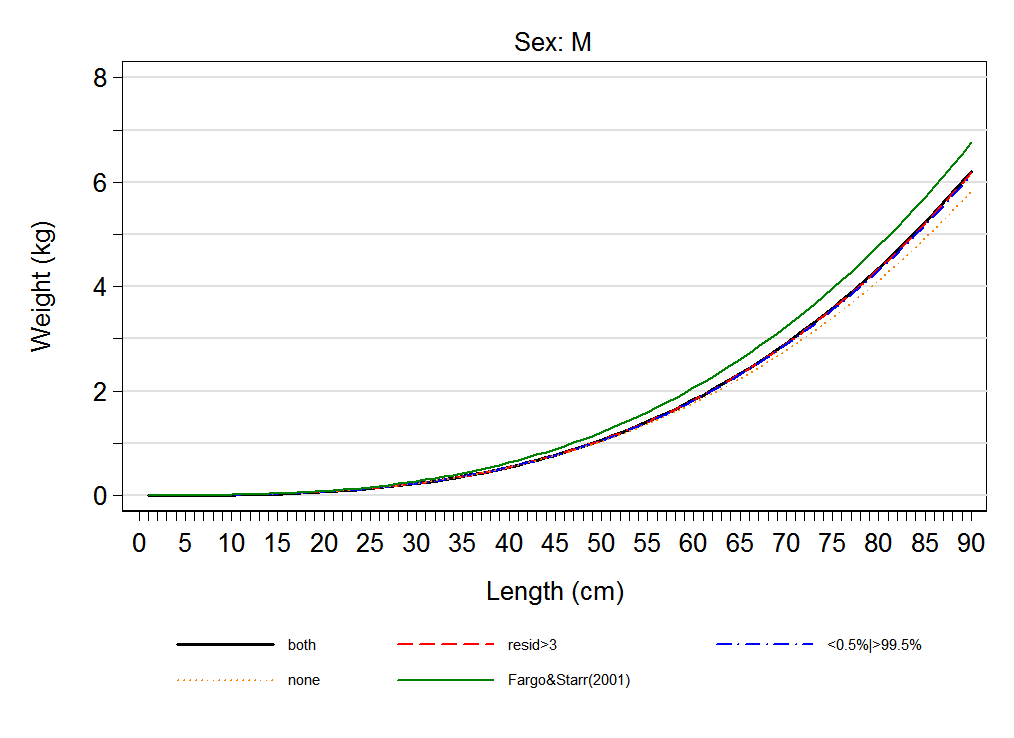
\includegraphics[bb=0 0 925 600,width=6in,keepaspectratio=true]{appD-Biology/lwmaleCompare.png}}
\newline
\subfloat[]{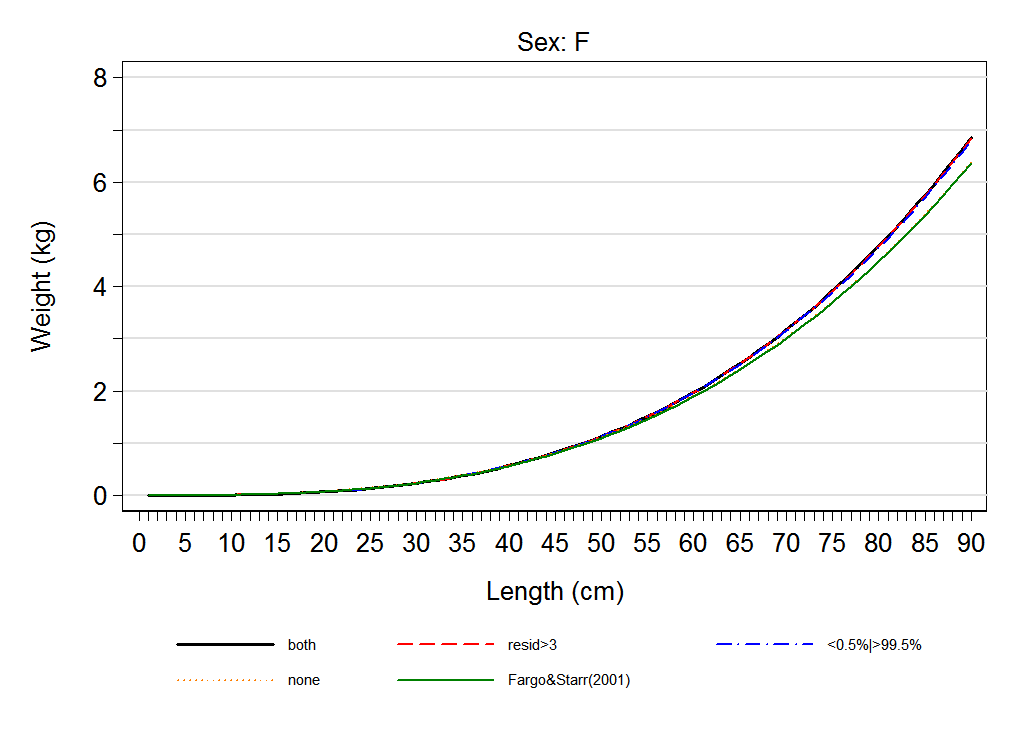
\includegraphics[bb=0 0 925 600,width=6in,keepaspectratio=true]{appD-Biology/lwfemaleCompare.png}}
\end{center}
\caption{Comparative length-weight plots for male [top panel] and female [bottom panel] \fishname, showing the predicted power functions for the four models defined in Table~\ref{tab:bioCrit}. Also shown is the function by sex provided in Table 2 of \citet{arf2001}.}
\label{fig:lwCompare}
\end{figure}

\begin{figure}[htp]
\captionsetup[subfigure]{labelformat=empty}
\begin{center}
\subfloat[]{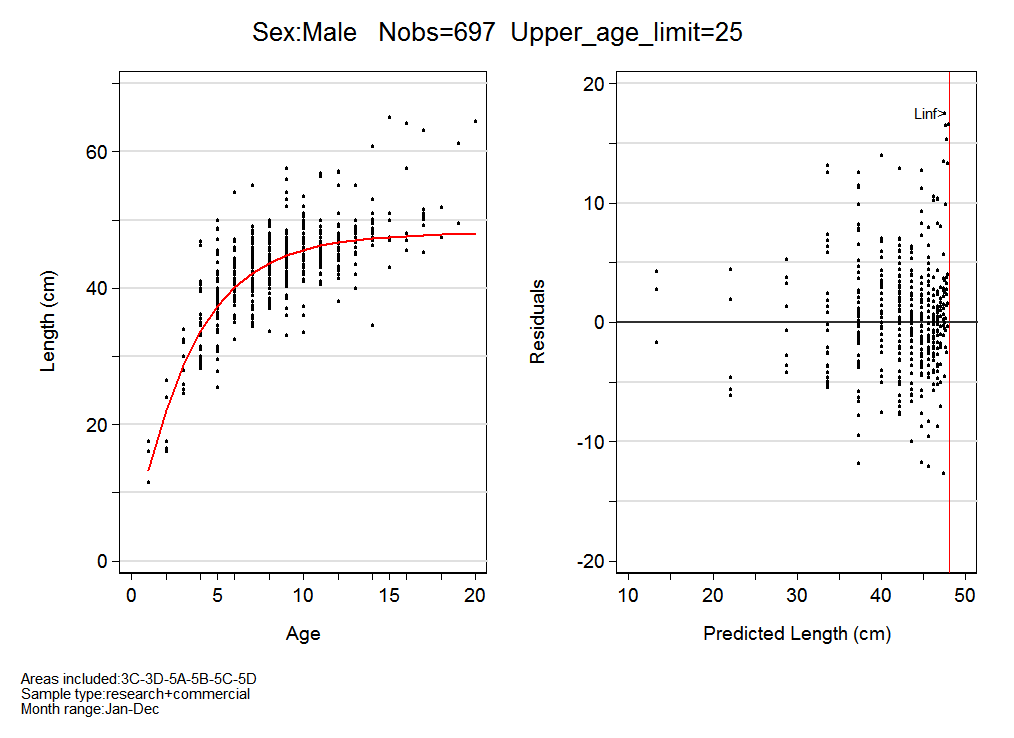
\includegraphics[bb=0 0 925 600,width=6in,keepaspectratio=true]{appD-Biology/vonbmale.png}}
\newline
\subfloat[]{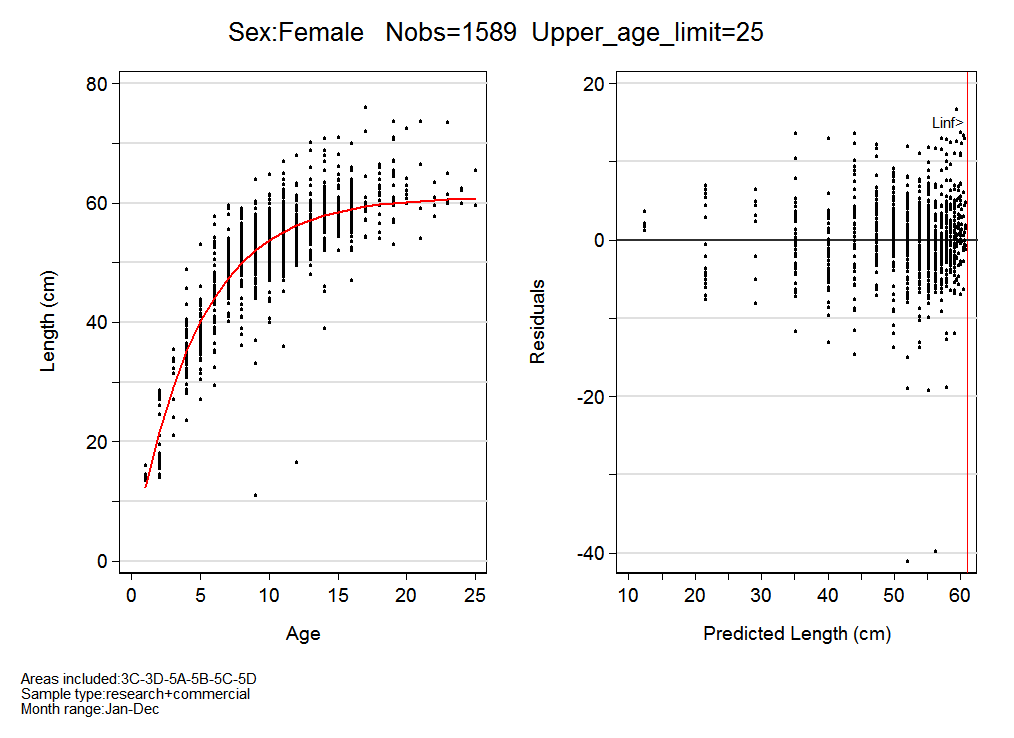
\includegraphics[bb=0 0 925 600,width=6in,keepaspectratio=true]{appD-Biology/vonbfemale.png}}
\end{center}
\caption{von-Bertalanffy plots for male [top panel] and female [bottom panel] \fishname: combined 3CD5ABCD using all available commercial and research data.}
\label{fig:vonb}
\end{figure}

\begin{figure}[htp]
\captionsetup[subfigure]{labelformat=empty}
\begin{center}
\subfloat[]{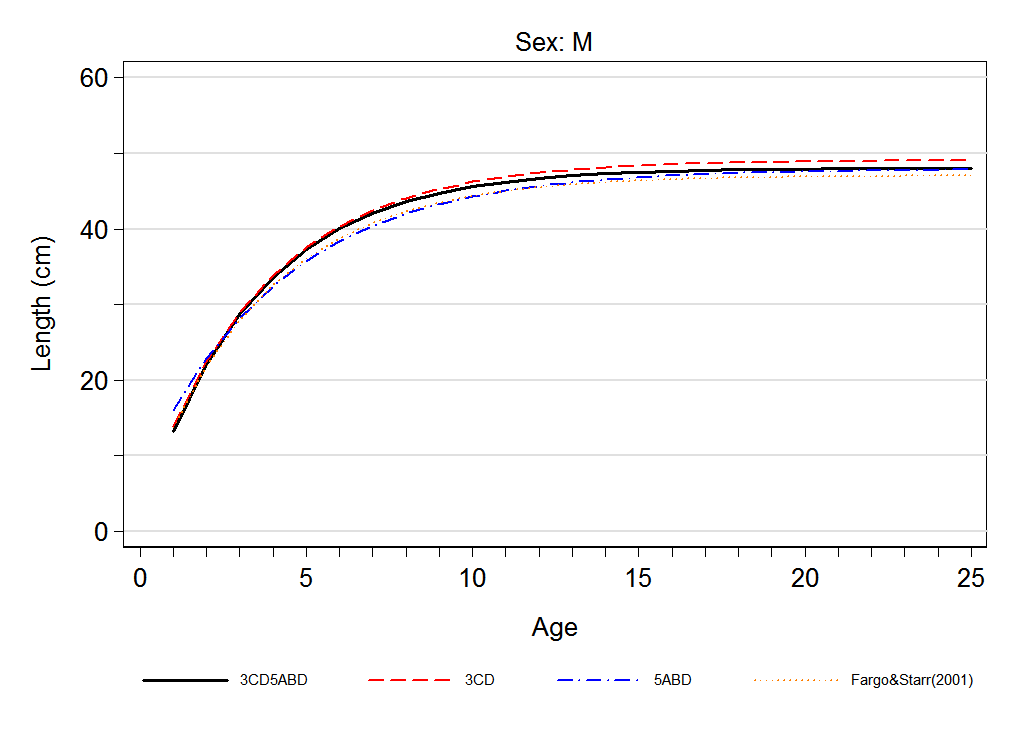
\includegraphics[bb=0 0 925 600,width=6in,keepaspectratio=true]{appD-Biology/vonbmaleCompare.png}}
\newline
\subfloat[]{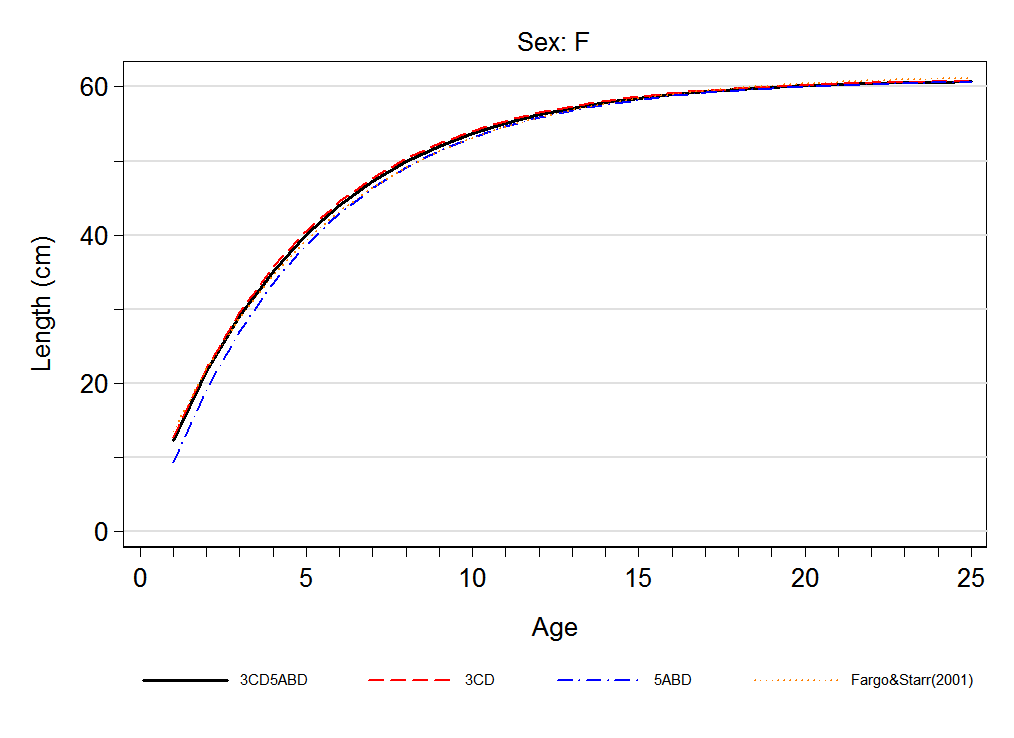
\includegraphics[bb=0 0 925 600,width=6in,keepaspectratio=true]{appD-Biology/vonbfemaleCompare.png}}
\end{center}
\caption{Comparative von-Bertalanffy plots for male [top panel] and female [bottom panel] \fishname, showing the predicted growth functions for the three models defined in Table~\ref{tab:vonbEst}.  Also shown is the function by sex provided in Table 2 of \citet{arf2001}.}
\label{fig:vonbCompare}
\end{figure}

\begin{figure}[htp]
\captionsetup[subfigure]{labelformat=empty}
\begin{center}
\subfloat[]{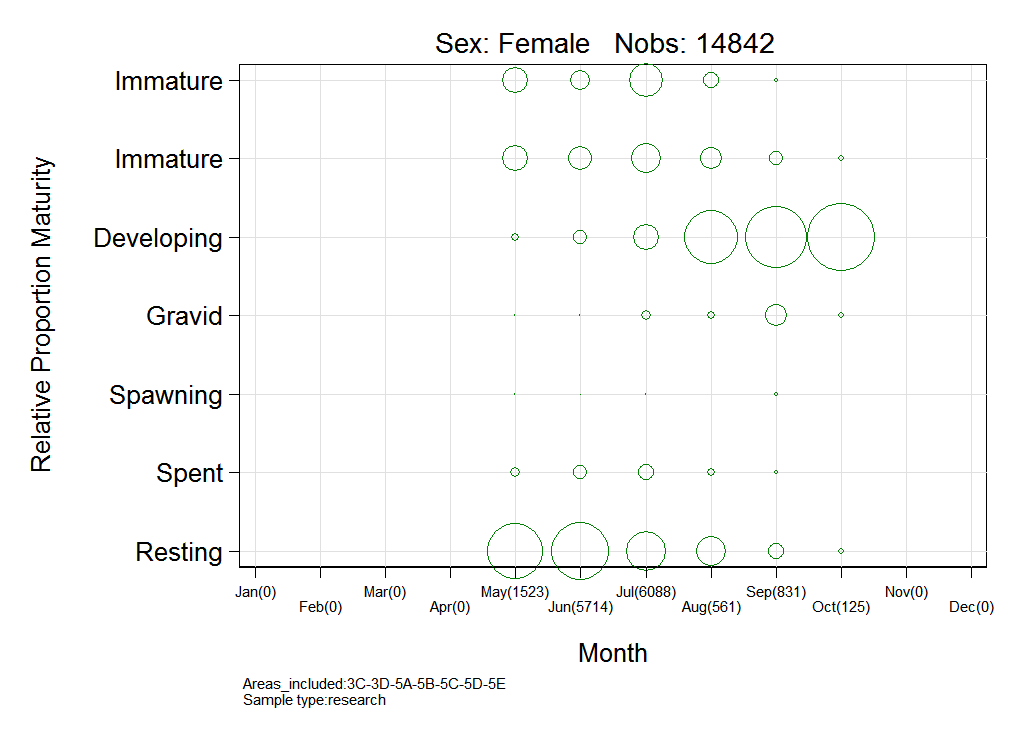
\includegraphics[bb=0 0 925 600,width=6in,keepaspectratio=true]{appD-Biology/maturityResearch.png}}
\newline
\subfloat[]{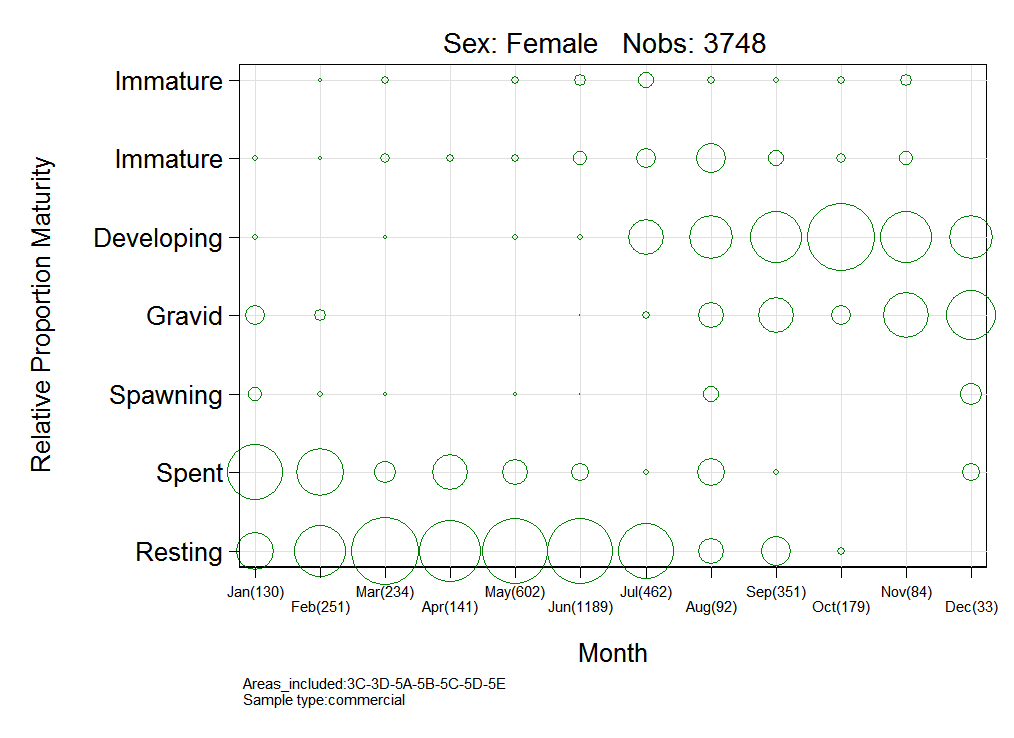
\includegraphics[bb=0 0 925 600,width=6in,keepaspectratio=true]{appD-Biology/maturityCommercial.png}}
\end{center}
\caption{Plots showing the proportion of \fishname females by maturity stage for each month; [top panel] research and charter survey observations [bottom panel] commercial observer observations. Each column sums to 1.0, with proportions provided in Table~\ref{tab:maturityMonth}}
\label{fig:maturity}
\end{figure}

\begin{figure}[htp]
\captionsetup[subfigure]{labelformat=empty}
\begin{center}
\subfloat[]{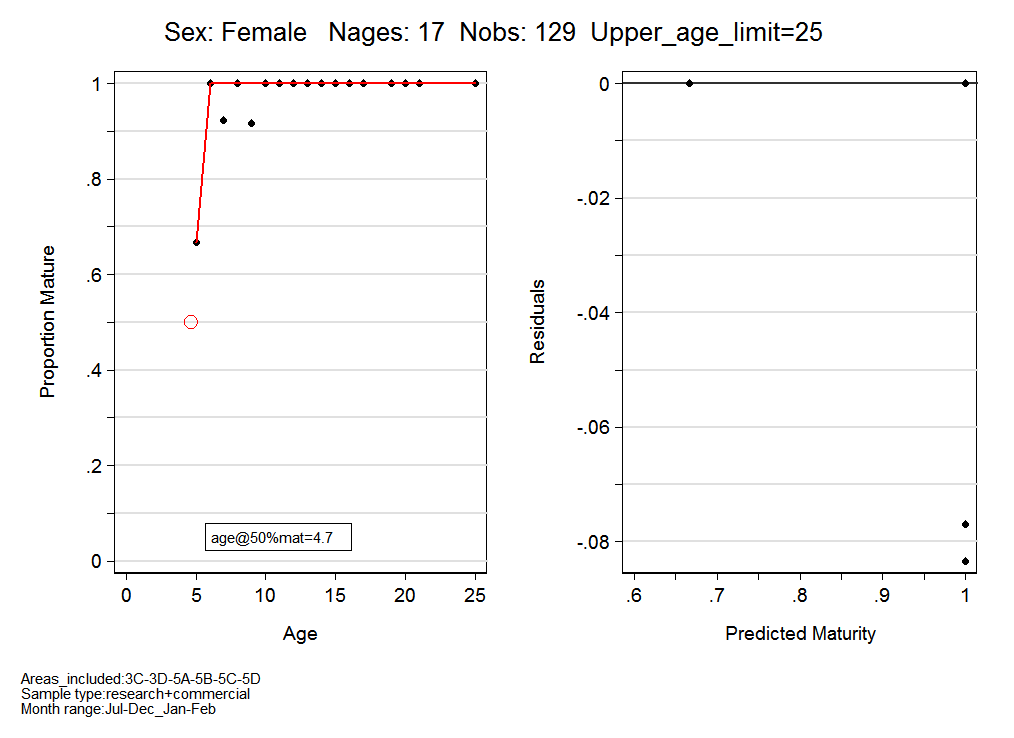
\includegraphics[bb=0 0 925 600,width=6in,keepaspectratio=true]{appD-Biology/maturityfitConstrainedMonths.png}}
\newline
\subfloat[]{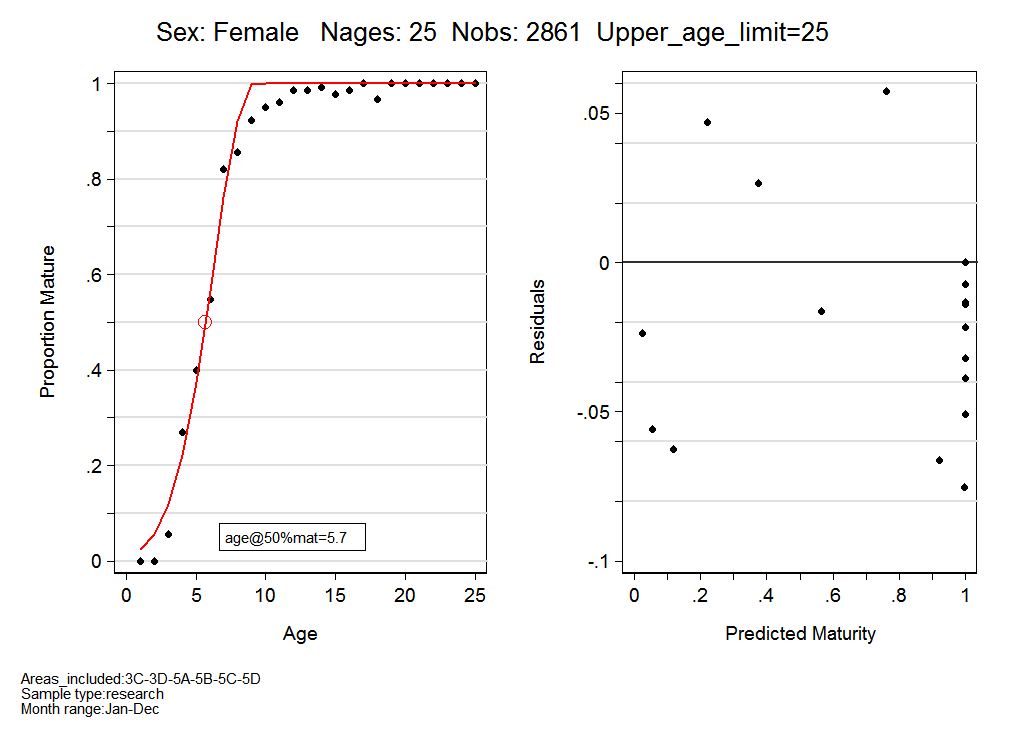
\includegraphics[bb=0 0 925 600,width=6in,keepaspectratio=true]{appD-Biology/maturityfitAllMonths.png}}
\end{center}
\vspace{-8mm}
\caption{Plots showing the observed proportions mature and the fitted maturity ogive by age for female \fishname: [top panel]: research and charter survey observations constrained to July-February; [bottom panel]: research observations from all months (January-November). The observed and fitted values by data source age, along with the number of otolith observations by age, are provided in Table~\ref{tab:maturityObsPred}.}
\label{fig:maturityfit}
\end{figure}

\begin{figure}[htp]
\captionsetup[subfigure]{labelformat=empty}
\begin{center}
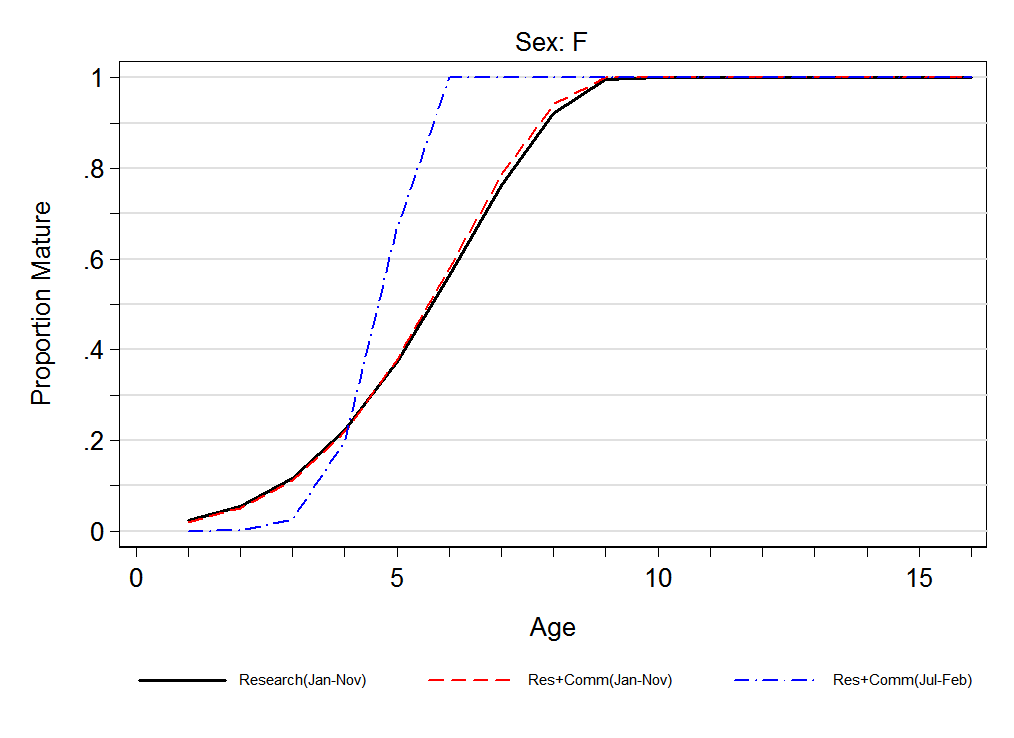
\includegraphics[bb=0 0 925 600,width=6in,keepaspectratio=true]{appD-Biology/maturityOgiveCompare.png}
\end{center}
\caption{Comparative maturity ogives for female \fishname, showing the predicted growth functions for the three models defined in Table~\ref{tab:parEst}.}
\label{fig:maturityOgiveCompare}
\end{figure}

\clearpage


% TABLES
\begin{table}[b]
\centering
\caption{\label{tab:bioCrit} Criteria for biological data extraction.}
\begin{tabular}{lrr}
\hline
Criterion & Notes \\
\hline
trip\_type==2 or trip\_type==3                               & definition of research observations \\
agemeth==3 or 17                                             & broken and burned or baked and broken \\
sample\_type==1 or 2 or 6 or 7                               & only random or total samples \\
month\textgreater=`startmonth' and month\textless=`endmonth' & valid month observation in range \\
sex==`sex'	                                                 & valid sex observation (1 or 2 ) \\
maturity\textgreater=1 and maturity\textless=7	             & valid maturity observation from 1 to 7 \\
select Not\_available\_reason\_code                          & not rejected \\
\hline
\end{tabular}
\end{table}

% To allow newlines in the table cells
\newcommand{\specialcell}[2][c]{%
  \begin{tabular}[#1]{@{}c@{}}#2\end{tabular}}

\begin{table}[b]
\tiny
\centering
\caption{\label{tab:lwEst} Length-weight parameter estimates, standard errors (SE) and number observations for male and female \fishname for all research observations in GFBio (trip\_type==2 or trip\_type==3) for combined PMFC Areas (3CD5ABCD) from 1989 to 2013. Restrictions are based on the distribution of residuals during a preliminary pass through data or on the empirical distribution of lengths by sex.}
\begin{tabular}{clcccccccc}
\hline
Option & Restrictions & \specialcell{N obs dropped\\residuals} & \specialcell{N obs dropped\\distribution} & \specialcell{N obs\\final} & $a^s$ & $b^s$ & SE($a^s$) & SE($b^s$) & $\bar{W}^s$ (kg) \\
\hline
Males \\
A & \specialcell{No distributional or residual\\restrictions} & 0 & 0 & 13,227 & -11.497 & 2.948 & 0.01600 & 0.00453 & 0.465 \\
B & \specialcell{No distributional restrictions\\residuals\textgreater3 dropped} & 79 & 0 & 13,148 & -11.714 & 3.009 & 0.00860 & 0.00243 & 0.465 \\
C & \specialcell{Lower 0.5\% and upper 99.5\%\\dropped, no residuals dropped} & 0 & 103 & 13,124 & -11.683 & 3.000 & 0.01121 & 0.00317 & 0.460 \\
D & \specialcell{Lower 0.5\% and upper 99.5\%\\dropped, residuals\textgreater3 dropped} & 127 & 103 & 12,997 & -11.732 & 3.014 & 0.00839 & 0.00237 & 0.461 \\
-- & \citet{arf2001} & -- & -- & -- & -11.270 & 2.930 & -- & -- & -- \\
\hline
Females \\
A & \specialcell{No distributional or residual\\restrictions} & 0 & 0 & 21,614 & -11.517 & 2.972 & 0.01560 & 0.00417 & 1.005 \\
B & \specialcell{No distributional restrictions\\residuals\textgreater3 dropped} & 55 & 0 & 21,559 & -11.871 & 3.066 & 0.00699 & 0.00186 & 1.005 \\
C & \specialcell{Lower 0.5\% and upper 99.5\%\\dropped, no residuals dropped} & 0 & 209 & 21,405 & -11.845 & 3.059 & 0.00883 & 0.00236 & 0.990 \\
D & \specialcell{Lower 0.5\% and upper 99.5\%\\dropped, residuals\textgreater3 dropped} & 168 & 209 & 21,237 & -11.890 & 3.071 & 0.00665 & 0.00177 & 0.992 \\
-- & \citet{arf2001} & -- & -- & -- & -11.600 & 2.993 & -- & -- & -- \\
\hline
\end{tabular}
\end{table}

\begin{table}[b]
\centering
\caption{\label{tab:numagesByArea} Number of paired length/observations by PMFC Region and sex. Also shows the maximum observed age by PMFC Region and sex.  Otoliths selected using criteria described in table~\ref{tab:bioCrit}.}
\begin{tabular}{lrrrr}
\hline
            & \multicolumn{2}{c}{Number ages} & \multicolumn{2}{c}{Maximum age} \\
\hline
PMFC region &  Male & Female &   Male & Female \\
\hline
3C          &   502 &    949 &     19 &     25 \\
3D          &   345 &    576 &     23 &     25 \\
5A          &     1 &      5 &     11 &     11 \\
5B          &    86 &    266 & 50$^1$ &     23 \\
5C          &   422 &    463 &     17 &     26 \\
5D          &   826 &  2,175 &     23 &     26 \\
5E          &    -- &     -- &     -- &     -- \\
Total       & 2,182 &  4,434 &     50 &     26 \\
$^1$ one observation only \\
\hline
\end{tabular}
\end{table}

\begin{table}[b]
\tiny
\centering
\caption{\label{tab:numagesByAreaMonth} Number of paired length/otolith observations by month and combined PMFC major region, showing the number of otoliths by sample source (Res=research or charter; Comm=observers aboard commercial vessels). Otoliths selected using criteria described in table~\ref{tab:bioCrit}.}
\begin{tabular}{|l|rrr|rrr|rrr|rrr|}
\hline
      & \multicolumn{3}{r|}{3CD} & \multicolumn{3}{r|}{5AB} & \multicolumn{3}{r|}{5CD} & \multicolumn{3}{r|}{Total Outside BC} \\
\hline
Month & Comm & Res & Total & Comm & Res & Total & Comm & Res & Total & Comm & Res & Total \\
\hline
January & 93 & -- & 93 & -- & -- & -- & -- & -- & -- & 93 & -- & 93 \\
February & 82 & -- & 82 & 1 & -- & 1 & -- & -- & -- & 83 & -- & 83 \\
March & 113 & -- & 113 & -- & -- & -- & 104 & -- & 104 & 217 & -- & 217 \\
April & 199 & -- & 199 & -- & -- & -- & -- & -- & -- & 199 & -- & 199 \\
May & 230 & 267 & 497 & 39 & -- & 39 & 404 & 354 & 758 & 673 & 621 & 1,294 \\
June & 223 & 1,051 & 1,274 & -- & 204 & 204 & 144 & 2,504 & 2,648 & 367 & 3,759 & 4,126 \\
July & 67 & -- & 67 & 30 & -- & 30 & 55 & -- & 55 & 152 & -- & 152 \\
August & -- & -- & -- & -- & -- & -- & -- & -- & -- & -- & -- & -- \\
September & -- & -- & -- & -- & -- & -- & 133 & -- & 133 & 133 & -- & 133 \\
October & 47 & -- & 47 & 49 & -- & 49 & 120 & -- & 120 & 216 & -- & 216 \\
Novermber & -- & -- & -- & 35 & -- & 35 & 68 & -- & 68 & 103 & -- & 103 \\
December & -- & -- & -- & -- & -- & -- & -- & -- & -- & -- & -- & -- \\
Total & 1,054 & 1,318 & 2,372 & 154 & 204 & 358 & 1,028 & 2,858 & 3,886 & 2,236 & 4,380 & 6,616 \\
\hline
\end{tabular}
\end{table}

\begin{table}[b]
\centering
\caption{\label{tab:vonbEst} von-Bertalanffy parameter estimates, standard errors (SE) and number observations for male and female \fishname for three models investigated for growth rate. Models in bold are the preferred models (plotted in Figure~\ref{fig:vonb}). These 3 models are superimposed by sex for comparison in Figure~\ref{fig:vonbCompare}.}
\begin{tabular}{lrrrrrrrr}
\hline
Option & Region & Nobs & $L_{\infty}^s$ & $k^s$ & $t_0^s$ & SE($L_{\infty}^s$) & SE($k^s$) & SE($t_0^s$) \\
\hline
Males \\
\textbf{Res+Comm} & \textbf{3CD5ABCD} & \textbf{2,181} & \textbf{50.13} & \textbf{0.239} & \textbf{-0.629} & \textbf{0.400} & \textbf{0.0105} & \textbf{0.1434} \\
Res+Comm & 3CD              & 847   & 51.96 & 0.237 & -0.453 & 0.712 & 0.0172 & 0.2524 \\
Res+Comm & 5ABCD            & 1,334 & 49.45 & 0.226 & -0.913 & 0.507 & 0.0126 & 0.1880 \\
 --      & \citet{arf2001}  & --    & 47.10 & 0.278 & -0.234 &    -- & --     & -- \\
Females \\
\textbf{Res+Comm} & \textbf{3CD5ABCD} & \textbf{4,432} & \textbf{61.65} & \textbf{0.190} & \textbf{-0.533} & \textbf{0.287} & \textbf{0.0042} & \textbf{0.0781} \\
Res+Comm & 3CD              & 1,525 & 62.84 & 0.191 & -0.427 & 0.459 & 0.0067 & 0.1372 \\
Res+Comm & 5ABCD            & 2,907 & 60.91 & 0.190 & -0.589 & 0.358 & 0.0053 & 0.0958 \\
 --      & \citet{arf2001}  & --    & 61.70 & 0.192 & -0.278 & --    & --     & -- \\
\hline
\end{tabular}
\end{table}

\begin{table}[b]
\tiny
\centering
\caption{\label{tab:maturityMonth} Proportion by maturity stage for each month for female \fishname, summed across all years for combined 3CD5ABCDE for A) research and charter boat observations; and B) commercial fishery observer observations. Each column sums to 1.0 for a month and sample type.}
\begin{tabular}{lrrrrrrrrrrrrr}
\hline
Stage      &   Jan &   Feb &   Mar &   Apr &   May &   Jun &   Jul &   Aug &   Sep &   Oct &   Nov &   Dec &  Total \\
\hline
\textbf{A) Research Observations} \\
Immature   &    -- &    -- &    -- &    -- & 0.146 & 0.087 & 0.238 & 0.053 & 0.002 &    -- &    -- &    -- &     -- \\
Immature   &    -- &    -- &    -- &    -- & 0.154 & 0.128 & 0.195 & 0.107 & 0.036 & 0.008 &    -- &    -- &     -- \\
Developing &    -- &    -- &    -- &    -- & 0.011 & 0.042 & 0.145 & 0.615 & 0.807 & 0.976 &    -- &    -- &     -- \\
Gravid     &    -- &    -- &    -- &    -- & 0.001 & 0.000 & 0.021 & 0.016 & 0.095 & 0.008 &    -- &    -- &     -- \\
Spawning   &    -- &    -- &    -- &    -- & 0.001 & 0.000 & 0.000 &    -- & 0.005 &    -- &    -- &    -- &     -- \\
Spent      &    -- &    -- &    -- &    -- & 0.018 & 0.040 & 0.057 & 0.012 & 0.004 &    -- &    -- &    -- &     -- \\
Resting    &    -- &    -- &    -- &    -- & 0.669 & 0.702 & 0.343 & 0.196 & 0.051 & 0.008 &    -- &    -- &     -- \\
N obs      &    -- &    -- &    -- &    -- & 1,577 & 6,171 & 6,088 &   561 &   831 &   125 &    -- &    -- & 15,353 \\
\hline
\textbf{B) Commercial Fishery Observations} \\
Immature   &    -- & 0.004 & 0.013 &    -- & 0.010 & 0.030 & 0.045 & 0.011 & 0.006 & 0.011 & 0.024 &    -- &     -- \\
Immature   & 0.008 & 0.004 & 0.017 & 0.014 & 0.013 & 0.042 & 0.076 & 0.163 & 0.051 & 0.022 & 0.036 &    -- &     -- \\
Developing & 0.008 &    -- & 0.004 &    -- & 0.008 & 0.007 & 0.253 & 0.380 & 0.527 & 0.877 & 0.536 & 0.364 &     -- \\
Gravid     & 0.069 & 0.032 &    -- &    -- &    -- & 0.001 & 0.011 & 0.120 & 0.248 & 0.078 & 0.405 & 0.485 &     -- \\
Spawning   & 0.038 & 0.008 & 0.004 &    -- & 0.003 & 0.001 &    -- & 0.054 &    -- &    -- &    -- & 0.091 &     -- \\
Spent      & 0.592 & 0.438 & 0.098 & 0.248 & 0.135 & 0.068 & 0.006 & 0.152 & 0.006 &    -- &    -- & 0.061 &     -- \\
Resting    & 0.285 & 0.514 & 0.863 & 0.738 & 0.831 & 0.851 & 0.608 & 0.120 & 0.162 & 0.011 &    -- &    -- &     -- \\
N obs      &   130 &   251 &   234 &   141 &   602 & 1,189 &   462 &    92 &   351 &   179 &    84 &    33 &  3,748 \\
\hline
\end{tabular}
\end{table}

\begin{table}[b]
\centering
\caption{\label{tab:maturityObsPred} Number of otoliths, observed and predicted maturities for the models (described in Table~\ref{tab:parEst}.) fitted to July--February and January--March.}
\begin{tabular}{|c|rrr|rrr|}
\hline
      & \multicolumn{3}{r|}{Res+Comm (Jul-Feb)} & \multicolumn{3}{r|}{Research (Jan-Nov)} \\
\hline
Age        & N\_otoliths & Obs\_mat & Pred\_mat & N\_otoliths & Obs\_mat & Pred\_mat \\
\hline
1  & -- &    -- &    -- &   6 &     0 & 0.024 \\
2  & -- &    -- &    -- & 121 &     0 & 0.056 \\
3  & -- &    -- &    -- &  91 & 0.055 & 0.117 \\
4  & -- &    -- &    -- & 108 & 0.269 & 0.221 \\
5  &  3 & 0.667 & 0.667 & 105 & 0.400 & 0.374 \\
6  &  2 &     1 &     1 & 126 & 0.548 & 0.564 \\
7  & 13 & 0.923 &     1 & 194 & 0.820 & 0.762 \\
8  & 12 &     1 &     1 & 318 & 0.855 & 0.922 \\
9  & 12 & 0.917 &     1 & 347 & 0.922 & 0.998 \\
10 & 20 &     1 &     1 & 374 & 0.949 &     1 \\
11 & 20 &     1 &     1 & 283 & 0.961 &     1 \\
12 & 12 &     1 &     1 & 213 & 0.986 &     1 \\
13 & 10 &     1 &     1 & 146 & 0.986 &     1 \\
14 & 13 &     1 &     1 & 137 & 0.993 &     1 \\
15 &  1 &     1 &     1 &  92 & 0.978 &     1 \\
16 &  3 &     1 &     1 &  74 & 0.986 &     1 \\
17 &  2 &     1 &     1 &  31 &     1 &     1 \\
18 &  2 &     1 &     1 &  31 & 0.968 &     1 \\
19 &  1 &     1 &     1 &  21 &     1 &     1 \\
20 &  2 &     1 &     1 &  19 &     1 &     1 \\
\hline
\end{tabular}
\end{table}

\begin{table}[b]
\centering
\caption{\label{tab:parEst} Parameter estimates with standard errors for three “double normal” models fitted to proportion mature by age fitting only the left-hand side variance and the age of full maturity (right-hand variance fixed such that maturity stays = 1.0. Also shown are the total number of otolith observations in each model and the derived parameter of median age of maturity ($^{50\%}a^f$).}
\begin{tabular}{llrrrrrr}
\hline
Data source & Month range & N\_otoliths & $A^f$ & ${\upsilon}L^f$ & SE($A^f$) & SE(${\upsilon}L^f$) & $^{50\%}a^f$ \\
\hline
Res+Comm    &     Jul-Feb &         129 &  6.00 &         0.903 &   0.0524 &            0.0000 &       4.69 \\
Res+Comm    &     Jan-Dec &       3,339 &  8.99 &         2.798 &   0.2259 &            0.1290 &       5.62 \\
Res         &     Jan-Nov &       2,861 &  9.21 &         2.891 &   0.2454 &            0.1336 &       5.68 \\
\hline
\end{tabular}
\end{table}

\clearpage
